% --
% spectrogram

\section{Spectral Features}\label{sec:signal_spec}
\thesisStateReady
Spectral features, such as a spectrogram, are the most intuitive form to represent audio waveforms. 
It is possible to observe active energy regions of certain frequency bands that are active at consecutive time chunks.
Methodically this is done by shifting an \emph{analytic window} of time span $t_N$, on the time axis.
The time shifting has also a fixed time interval, denoted as \emph{hop time} $t_{h}$.
Both time parameters $t_N$ and $t_h$ can also be presented in samples through a multiplication with the sampling frequency $f_s$:
% --
% samples
\begin{equation}
  \begin{split}
    N &= t_N \, f_s, \\
    h &= t_h \, f_s.
  \end{split}
\end{equation}
The audio samples contained by the analytic window of size $N$, are transformed with the Discrete Fourier Transform (DFT):
% --
% DTFT
\begin{equation}\label{eq:signal_spec_dtft}
  \hat{X}[k] = \sum_{n=0}^{N-1} x[n] \, e^{-j\frac{2 \pi n}{N}k}
\end{equation}
into the frequency space $\hat{X}[k] \in \C$ with frequency index $k$ and discrete audio samples $x[n]$ with sample index $n$.
More conveniently, \req{signal_spec_dtft} can be written in matrix notation with the DFT operator denoted as $\mathcal{F} \in \C^{N \times K}$ with a total number of $N$ samples of the input signal $x \in \R^N$ and $K$ Fourier coefficients:
%--
% DFT matrix
\begin{equation}\label{eq:signal_spec_dtft_matrix}
  \hat{X} = x^T \, \mathcal{F} \quad \mathrm{with} 
  \quad \mathcal{F}[n, k] = e^{-j\frac{2 \pi n}{N} k},
  \quad n,\, k = (0, 1, \dots N-1),\, (0, 1 \dots K-1)
\end{equation}
where $n$ and $k$ are row and column indices in the matrix $\mathcal{F}$, which gives an output dimension of the DFT $\hat{X} \in \C^K$.

The length of the analytic window in samples $N$ is crucial for the frequency resolution and the lowest frequency that can be represented.
For example, the periodic time of a sound with $f=\SI{20}{\hertz}$ is $t=\frac{1}{f} = \SI{50}{\milli\second}$.
To represent a waveform it is necessary to have at least a quarter of its wavelength captured.
Within this thesis, the length of the analytic window is selected to \SI{25}{\milli\second}, which is enough for speech signals.

The \emph{hop size} $h$ in samples of the hop time $t_h$, by which the analytical window is shifted on the time axis, indicates the resolution in time and is especially important for sequential changes within the audio data.
In applications like speech processing, the hop time should be selected so that the fastest pronounced phone and its transitions to other phones is captured with sufficient resolution.
Usually a hop time of $t_{h}=\SI{10}{\milli\second}$ is chosen for speech recognition tasks (also used within this thesis), but it could be extended to $t_{h}=\SI{20}{\milli\second}$, applied in \cite{Peter2020} to save computations.

With the hop size $h$ in samples and $N$ the length of the analytical window, the Short-Time Fourier Transform (STFT) for discrete time signals, can be computed as:
% --
% stft
\begin{equation}\label{eq:signal_spec_stft}
    \tilde{X}[m, k] = \sum_{n=0}^{N-1} x[n + m] \, w[n] \, e^{-j\frac{2 \pi n}{N}k}, \qquad m = 0 h, \, 1 h, \, \dots, \, M h 
\end{equation}
so that $\tilde{X}[m, k] \in \C$ is the STFT coefficient of frame $m$ and DFT coefficient $k$, where $n$ is denoted here as summation index, $w$ as a window function, such as the \emph{Hanning} window, $m$ indicates the frame index shifted by the hop size $h$ and $M$ is the maximum number of possible hops until the end of the signal is reached by shifting the analytical window of size $N$ by the hop size on the discrete time axis.
The maximum number of hops $M$ can therefore be computed as:
% --
% hop
\begin{equation}\label{eq:signal_spec_hop}
  M = \ceil*{\frac{n-N}{h}}
\end{equation}
where $n$ is here the length of the discrete time signal $x$.
The calculation of the STFT can be written in matrix notation if the input chunks from the shifting of the analytic window is denoted as vector:
\begin{equation}
  \bar{x}_i = [\, x_{i \cdot h}, \dots, x_{i \cdot h+N}]^T
\end{equation}
where each individual $\bar{x}_i \in \R^N$ can be concatenated in a matrix $X \in \R^{M \times N}$ denoted as:
\begin{equation}
  X = 
  \begin{bmatrix}
    \bar{x}_1^T \\
    \vdots\\
    \bar{x}_M^T \\
  \end{bmatrix}
\end{equation}
so that the STFT $\tilde{X} \in \C^{M \times K}$ can be conveniently written as:
% --
% stft matrix
\begin{equation}\label{eq:signal_spec_stft_matrix}
  \tilde{X} = X \, \diag{\bar{w}} \, \mathcal{F}
\end{equation}
where $\diag{\bar{w}}$ is a diagonal matrix of weight vectors with the window function written as vector $\bar{w} \in \R^N$.
The matrix $\tilde{X} \in \C^{M \times K}$ represents the whole STFT where the rows are the shifts of the analytical window on the time axis and the columns are the Fourier coefficients of each DFT.
The used STFT parameters for this thesis are shown in \rtab{signal_spec_stft}.
% --
% stft params
% --
% stft params
\begin{table}[ht!]
\begin{center}
\caption{Parameters used for the STFT computation.}
\begin{tabular}{ M{4cm}  M{4cm}}
\toprule
\textbf{Parameter} & \textbf{Value} \\
\midrule
Sampling Frequency & \SI{16}{\kilo\hertz}\\
Analytic window size & \SI{25}{\milli\second}\\
Hop size & \SI{10}{\milli\second}\\
Window Function & Hanning\\
\bottomrule
\label{tab:signal_spec_stft}
\end{tabular}
\end{center}
\vspace{-4mm}
\end{table}
\FloatBarrier
\noindent
A spectrogram $P \in \R^{M \times K}$ is simply the power spectrum of the STFT $\tilde{X} \in \C^{M \times K}$ computed as:
% --
% spec
\begin{equation}\label{eq:signal_spec_spec}
  P = \abs{\tilde{X}}^2.
\end{equation}
Note that $P$ has now real values instead of complex ones.
The recorded examples transformed to a spectrogram with linear representation is shown in \rfig{signal_spec_lin_showcase}.
\begin{figure}[!ht]
  \centering
    \subfigure[left]{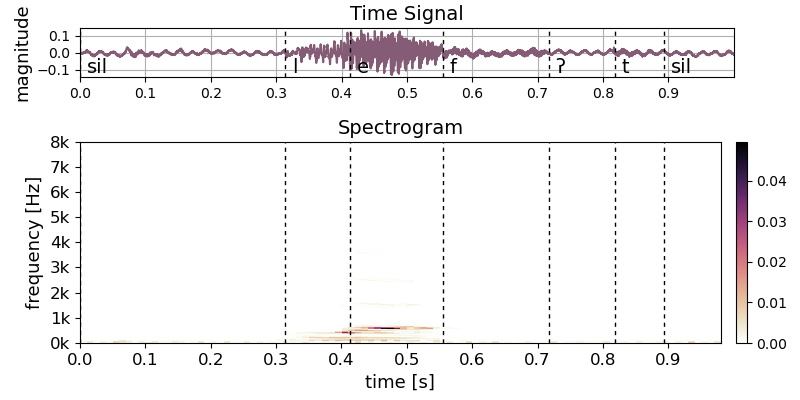
\includegraphics[width=0.45\textwidth]{./3_signal/figs/signal_spec-lin_showcase_left0}}
    \subfigure[right]{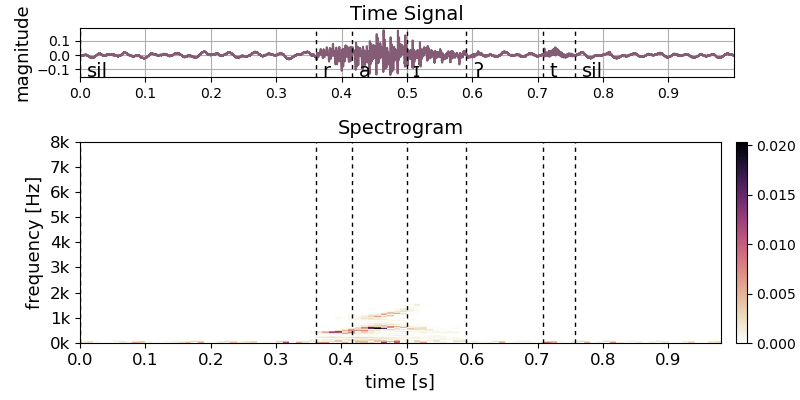
\includegraphics[width=0.45\textwidth]{./3_signal/figs/signal_spec-lin_showcase_right0}}
    \subfigure[up]{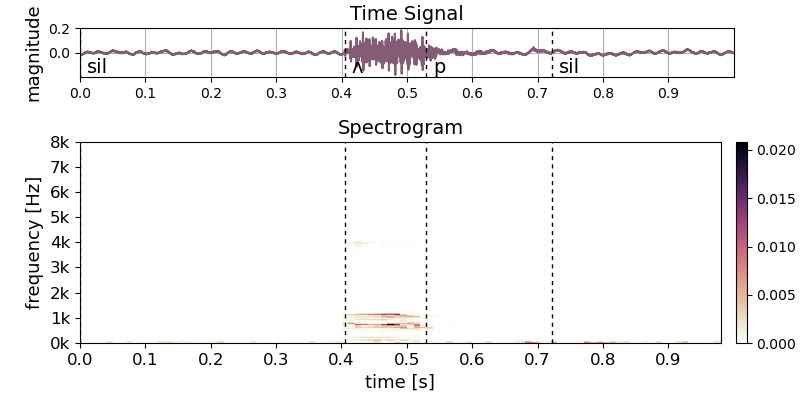
\includegraphics[width=0.45\textwidth]{./3_signal/figs/signal_spec-lin_showcase_up0}}
    \subfigure[down]{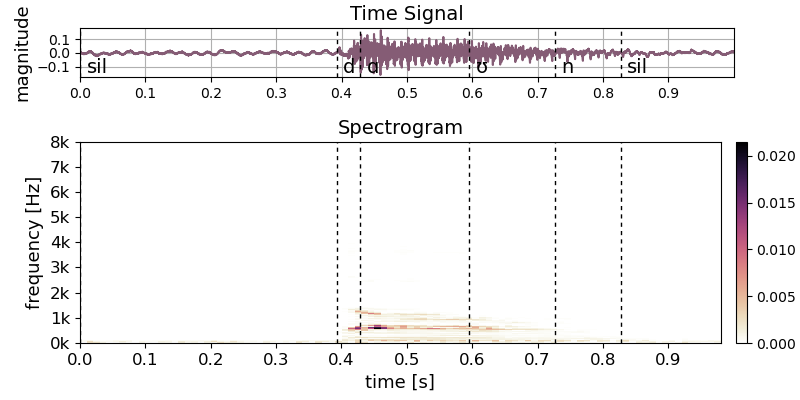
\includegraphics[width=0.45\textwidth]{./3_signal/figs/signal_spec-lin_showcase_down0}}
    \subfigure[go]{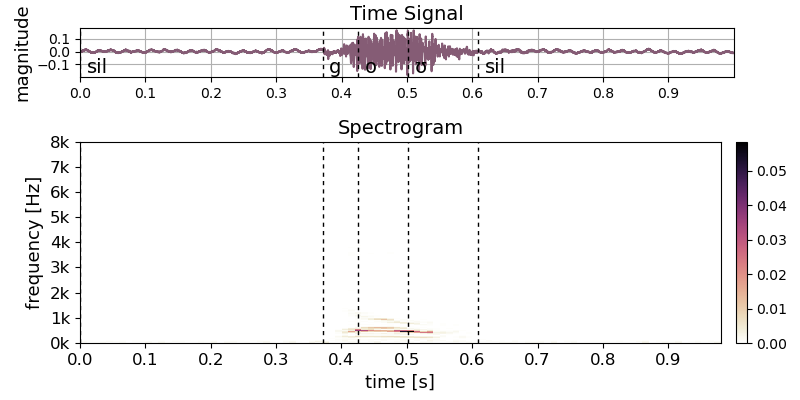
\includegraphics[width=0.45\textwidth]{./3_signal/figs/signal_spec-lin_showcase_go0}}
  \caption{Spectrogram linear scaled.}
  \label{fig:signal_spec_lin_showcase}
\end{figure}
\FloatBarrier
\noindent
It can be observed, that most of the signals energy is in the lower frequency regions of under approximately \SI{1}{\kilo\hertz}, therefore it is more appealing to transform the spectrogram into the log scale of its value space, achieved by:
% --
% log
\begin{equation}\label{eq:signal_spec_log}
  P_{DB} = 10 \cdot \log{P}
\end{equation}
so that small energies are more emphasized with $P_{DB} \in \R^{M \times K}$. 
The same examples with log scaling in the value space visualized with log scaling of the frequency space in the plots are shown in \rfig{signal_spec_log_showcase}.
\begin{figure}[!ht]
  \centering
    \subfigure[left]{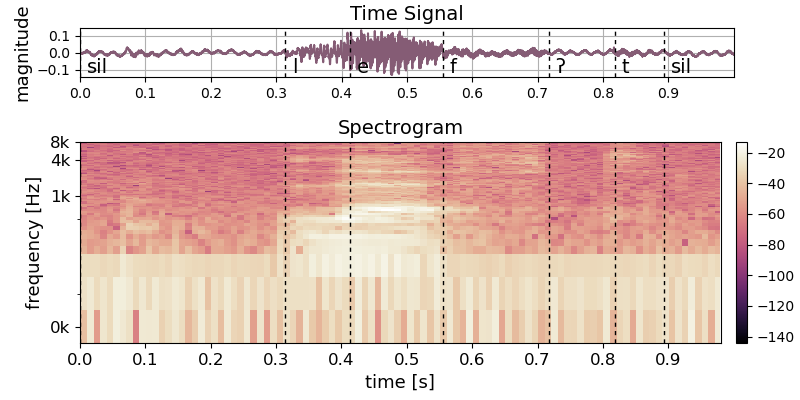
\includegraphics[width=0.45\textwidth]{./3_signal/figs/signal_spec-log_showcase_left0}}
    \subfigure[right]{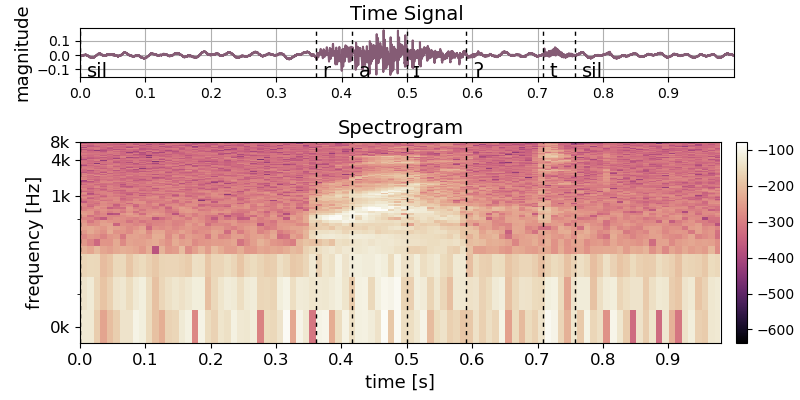
\includegraphics[width=0.45\textwidth]{./3_signal/figs/signal_spec-log_showcase_right0}}
    \subfigure[up]{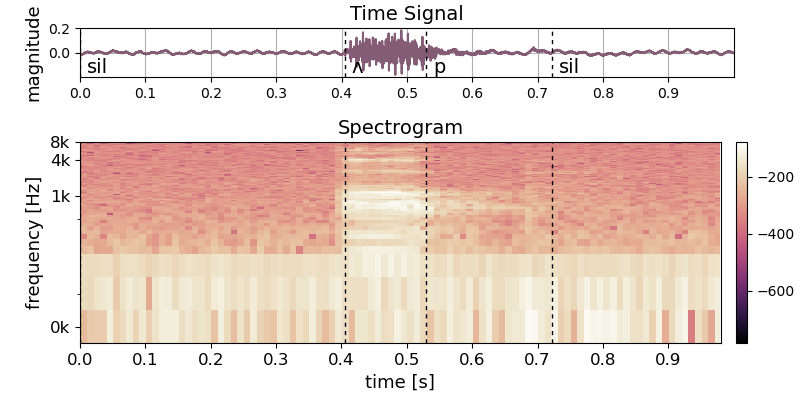
\includegraphics[width=0.45\textwidth]{./3_signal/figs/signal_spec-log_showcase_up0}}
    \subfigure[down]{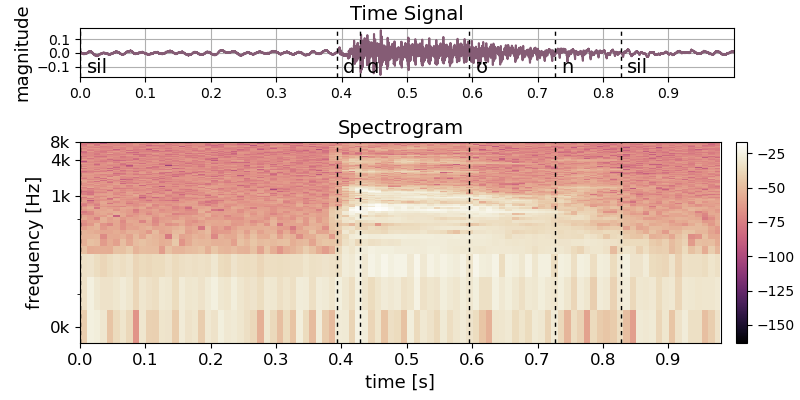
\includegraphics[width=0.45\textwidth]{./3_signal/figs/signal_spec-log_showcase_down0}}
    \subfigure[go]{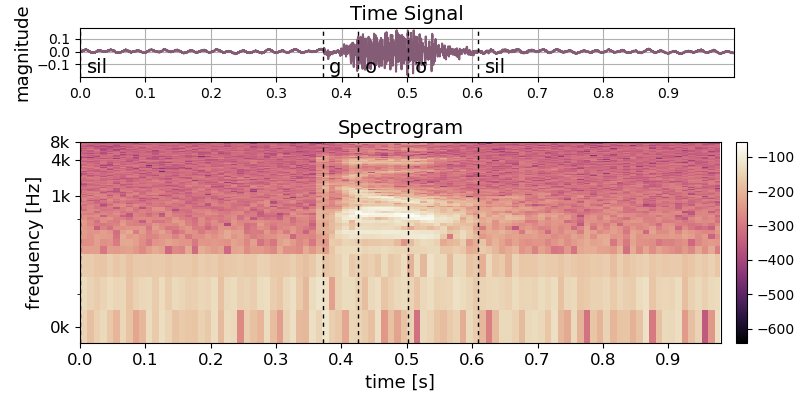
\includegraphics[width=0.45\textwidth]{./3_signal/figs/signal_spec-log_showcase_go0}}
  \caption{Spectrogram logarithmic scaled.}
  \label{fig:signal_spec_log_showcase}
\end{figure}
\FloatBarrier
\noindent
It is now possible to observe some interesting structures and movements in certain frequency bands over time.
A compression scheme, such as the Mel Frequency Cepstral Coefficients (MFCC) explained in the next section, reduces the high dimensional frequency feature vectors of the STFT to more compact feature vectors and further improves the visualization of the spoken command words.